\documentclass[11pt,a4paper]{article}
\usepackage[utf8]{inputenc}
\usepackage[T1]{fontenc}
\usepackage{mathptmx}
\usepackage{amsfonts}
\usepackage{amsmath, amssymb}
\usepackage{bm}
\usepackage{nccmath}
\usepackage{graphicx}
\usepackage{titling}
\usepackage{indentfirst}
\usepackage{url}
\usepackage{xurl}
\usepackage[backend=biber,style=apa,date=year]{biblatex}
\usepackage{csquotes}
\usepackage{float}
\usepackage{sectsty}
\usepackage{enumitem}
\usepackage{hyphenat}
\usepackage{wrapfig}
\usepackage{hyperref}
\usepackage{enumitem}
\usepackage{titlesec}
\usepackage[skip=0pt]{caption}
\setlength{\parskip}{1em}
\usepackage{tikz}
\usepackage{breakcites}
\usetikzlibrary{positioning}
\usepackage{geometry}
\usepackage{makecell}
 \geometry{
 a4paper,
 left=25.4mm,
 right=25.4mm,
 top=25.4mm,
 bottom=25.4mm
 }
\usepackage{subcaption}


\hypersetup{
    colorlinks=TRUE, %set true if you want colored links
    linktoc=all,     %set to all if you want both sections and subsections linked
    citecolor=blue,
    linkcolor=blue,
    urlcolor=blue%choose some color if you want links to stand out
}
\DeclareSourcemap{
  \maps[datatype=bibtex]{
      \map{
        \step[fieldset=urldate, null]
      }
   }
}
\usepackage[top=0.5in, bottom=0.5in,left=1in,right=1in]{geometry} 
\addbibresource{Bio.bib}

%%%%%%%%%%%%%%%%%%%%%%%%%%%%%%%%%%%%%%%%%%%%%%%%%%%%%%%%%%%%%%%%%%%%%%%%%%%%%%%%%%%%%%%%%%%%%%%%%%%%%%%%%%%%



\title{Balancing Groundwater Sustainability and Agricultural Economic Goals through Evolutionary Direct Policy Search}

\author{José M. Rodríguez-Flores, Rohini Gupta, Harrison B. Zeff, Patrick M. Reed, Josué Medellín-Azuara}

\date{}

\begin{document}

\maketitle


\section*{Abstract}

The framework used in this study enables us to find policy strategies that are more likely accepted by stakeholders due to the heterogeneity of solutions in the Pareto-set and their robustness to uncertain surface water supplies. 
 
\section{Introduction}

As irrigation water demand increases and droughts become more frequent, agricultural regions in the world are relying more on groundwater. In Mediterranean climate regions, as California, and arid and semi-arid regions with variable precipitation, groundwater is a reliable source of water and key for water security and food security (\cite{priyan_issues_2021,malmgren_groundwater_2022}). Aquifer systems flux dynamics are sensitive to changes in temperatures, precipitation and surface water flows, that are impacted with climate change (\cite{w,cuthbert_global_2019}). However the largest impact from climate change is indirectly through changes in land use and water demand by human activities (\cite{taylor_ground_2013}). Globally water from aquifers account for 43 percent of the total irrigation (\cite{siebert_groundwater_2010}), which is expected to increase as surface water scarcity increases (\cite{wada_nonsustainable_2012}). Additionally the lack of groundwater management in agriculture have lead to stress and depletion of aquifers (\cite{dalin_groundwater_2017, wada_global_2010}), affecting dependant ecosystems (\cite{bierkens_non-renewable_2019}), limiting its access to shallow water-table reliant communities (\cite{perrone_dry_2017,pauloo_domestic_2020}), reducing groundwater quality, among others. For this reason groundwater management and long-term planing is necessary to stop the groundwater depletion trajectory that has been observed globally (\cite{gorelick_global_2015}).

Multiple challenges inherent to coupled food-water systems (\cite{polhill_modelling_2016}) are present in groundwater management. First, food-water systems are dynamic, each component evolve as well as their feed-backs (\cite{filatova_regime_2016}), thus management decisions should adapt as the coupled system evolves. Second, water management policies may result in trade-offs between economic and sustainability objectives (\cite{mcdermid_minimizing_2021,torhan_tradeoffs_2022,young_hydrologic-economic_2021,stone_economic_2022}). Lastly, there are intrinsic uncertainties sometimes considered deep uncertainties or with no knowledge of their distribution (\cite{stirling_keep_2010}) that need to be accounted, including uncertain surface water supplies, crop prices, among others.  

There is a growing literature on assessing management policies and mechanisms for groundwater sustainability in agriculture. Water use and land use controls as well as economic instruments are the most common strategies that have been studied, such as groundwater pumping taxing and pricing (\cite{madani_exogenous_2013,mulligan_assessing_2014,stone_economic_2022}), pumping restrictions (\cite{young_hydrologic-economic_2021,lan_performance_2021,macewan_hydroeconomic_2017,rodriguez-flores_global_2022}), pricing energy (\cite{hrozencik_impacts_2022}), groundwater markets or trading mechanisms (\cite{khan_effect_2019,kuwayama_regulation_2013}), land fallowing (\cite{van_schmidt_linkages_2022}), land management (\cite{bourque_balancing_2019,li_evaluation_2018,bryant_shaping_2020}) and the combination of different strategies (\cite{graveline_combining_2019,hrozencik_heterogeneous_2017}). However most of the studies do not capture the complexity in the decision making  and do not take into account intrinsic uncertainties as surface water supplies change every year and management decisions may change between wet and dry periods. 

Recent modeling frameworks show the benefits of dynamic adaptive policies in complex systems (\cite{herman_climate_2020,walker_adapt_2013}), able to  represent the adaptive capacity in management decisions under uncertainty.  Adaptive policy modeling frameworks, such as Evolutionary Multi-objective Direct Policy Search (EMODPS) (\cite{giuliani_curses_2016,macian-sorribes_inferring_2019}) have been applied to other complex water management decisions, as reservoir operation and financial portfolios (\cite{zatarain_salazar_balancing_2017,gupta_can_2020}). EMODPS as a Direct Policy Search (DPS) framework relies on a parameterization-simulation-optimization (\cite{koutsoyiannis_evaluation_2003}) process where the structural parameters of a non-linear network are optimized using Multi-objective Evolutionary Algorithms (MOEA), rather than the policy decisions. This process reduces the "course of dimensionality" of other dynamic frameworks as Stochastic Dynamic Programming applied in agriculture (\cite{taylor_dynamic_1993}). 

The resulting control policy can map information variables of the system (e.g surface water available, groundwater depth and irrigation demand) to inform policy decisions showing a feed-back or closed loop control resulting in state-aware policies. Additionally, this framework is suitable to multi-objective problems, where the MOEA optimization results in a pareto-set of solutions (\cite{coello_evolutionary_2007}) that span a space with trade-offs among objectives (e.g economic revenues and groundwater depth) from sustainable groundwater management (\cite{greening_design_2004,null_pareto_2021}). Lastly, studies that search for optimal groundwater management policies generally focus on one policy at a time, that does not represent the possible suit of decisions that water managers and farmers can perform to achieve groundwater sustainability. The flexibility of the control policy in the EMODPS formulation offers the possibility to include a set of management decisions that can be implemented simultaneously every time step. Furthermore, policies found in the Pareto-set can be assessed to find policies that perform well under multiple system state conditions or states of the world (SOWs) (\cite{herman_climate_2020}), including surface water delivers and crop prices, based  on potential stakeholders preferences. This is done by following Robust Decision Making (RDM) framework (\cite{lempert_making_2013,groves_robust_2019}) to identify the policies that perform the best under uncertain futures. This is done by using different acceptability criteria to find robust policies (\cite{mcphail_robustness_2018}). This framework has been widely used to asses the ability of water management polices to address water demand, economic and sustainability objectives under uncertainty \cite{miro_adaptive_2021,graveline_combining_2019,quinn_direct_2017}.

This study shows a novel application of combined hydro-economic and heuristic methods using a Bi-level optimization process where an agricultural production model with a groundwater depth response function is nested in a MOEA to find adaptive management policies to achieve groundwater sustainability. This modeling framework is applied to the Semitropic Water Storage District in the San Joaquin Valley, California where there is an ongoing development and implementation of strategies to address groundwater sustainability mandated by state legislation. The objectives of this study are twofold. First, asses the ability of EMODPS to identify adaptive strategies that achieve groundwater sustainability and economic goals accounting for the characteristics of the food-water system. Second, asses the performance of the optimal policies within the context of the sustainable groundwater management criteria defined by the state and the trade-offs between groundwater sustainability and economic revenues from food production. 

\section{Study area and problem definition}

The San Joaquin Valley (SJV) in California is the most important agricultural region in the United States by economic value (\cite{usda_national_2020}). The Mediterranean weather in the region and its dependence on atmospheric rivers that supplies precipitation and snow-pack make it vulnerable to drought events (\cite{espinoza_global_2018}). Additionally, increments on temperature, evapotranspiration, and reduced surface water supply are expected to exacerbate with climate change (\cite{fernandez-bou_regional_2021}).

During the past decade the agricultural sector has been largely impacted by multi-year droughts (\cite{lund_lessons_2018,medellin-azuara_economic_2022}). Groundwater pumping is used as a buffer to reduce the negative impacts to agricultural production from surface water shortages, but increasing pumping, reduced groundwater recovery and lack of management have led to overdraft  (\cite{liu_groundwater_2022}). Negative effects from groundwater depletion, include land subsidence (\cite{ojha_sustained_2018}), lowering groundwater levels, reduction of groundwater storage (\cite{alam_post-drought_2021}), and degraded water quality (\cite{levy_critical_2021}). Additionally, in the SJV there has been an expansion of perennial tree crops, mainly Almonds which is the most important commodity by value  in the region (\cite{usda_national_2020}). Although high profitable, the expansion of perennial tree crops represents a less flexible water demand and a higher financial risk to water shortages due to high establishment costs (\cite{qin_flexibility_2019,mall_water_2019}). Other important commodities in the region include vine, alfalfa, corn, cotton and cucumbers (SI Figure S1). 

\subsection{Sustainable Groundwater Management}

 The Sustainable Groundwater Management Act (SGMA) (\cite{dwr_sustainable_2021}), released in 2014, requires critically over-drafted basins to achieve sustainable groundwater management by 2040. Groundwater Sustainability Agencies (GSAs) are responsible to develop and enforce policies to manage the conjunctive use of water to address groundwater sustainability goals, including a sustainable groundwater level. The state defined  guidelines in the Sustainable Management Criteria (\cite{dwr_sustainable_2017}) that GSAs can use to develop management strategies. The sustainable criteria defines a margin of operational flexibility where the groundwater depth can go above the measurable objective but not beyond the minimum threshold where undesirable results may ocurr, as shown by Figure 1. With this framework GSAs can develop flexible groundwater management strategies, allowing pumping during dry years and maximizing groundwater recharge during wet years. Furthermore, food production needs to adapt water and land allocation decisions, as well as crop choice, to achieve groundwater sustainability goals and be less vulnerable to surface water shortages. As mentioned in the introduction one of the objectives of this study is to identify adaptive policies and provide insight within the context of the sustainable criteria.

 \begin{figure}[H]
    \centering
    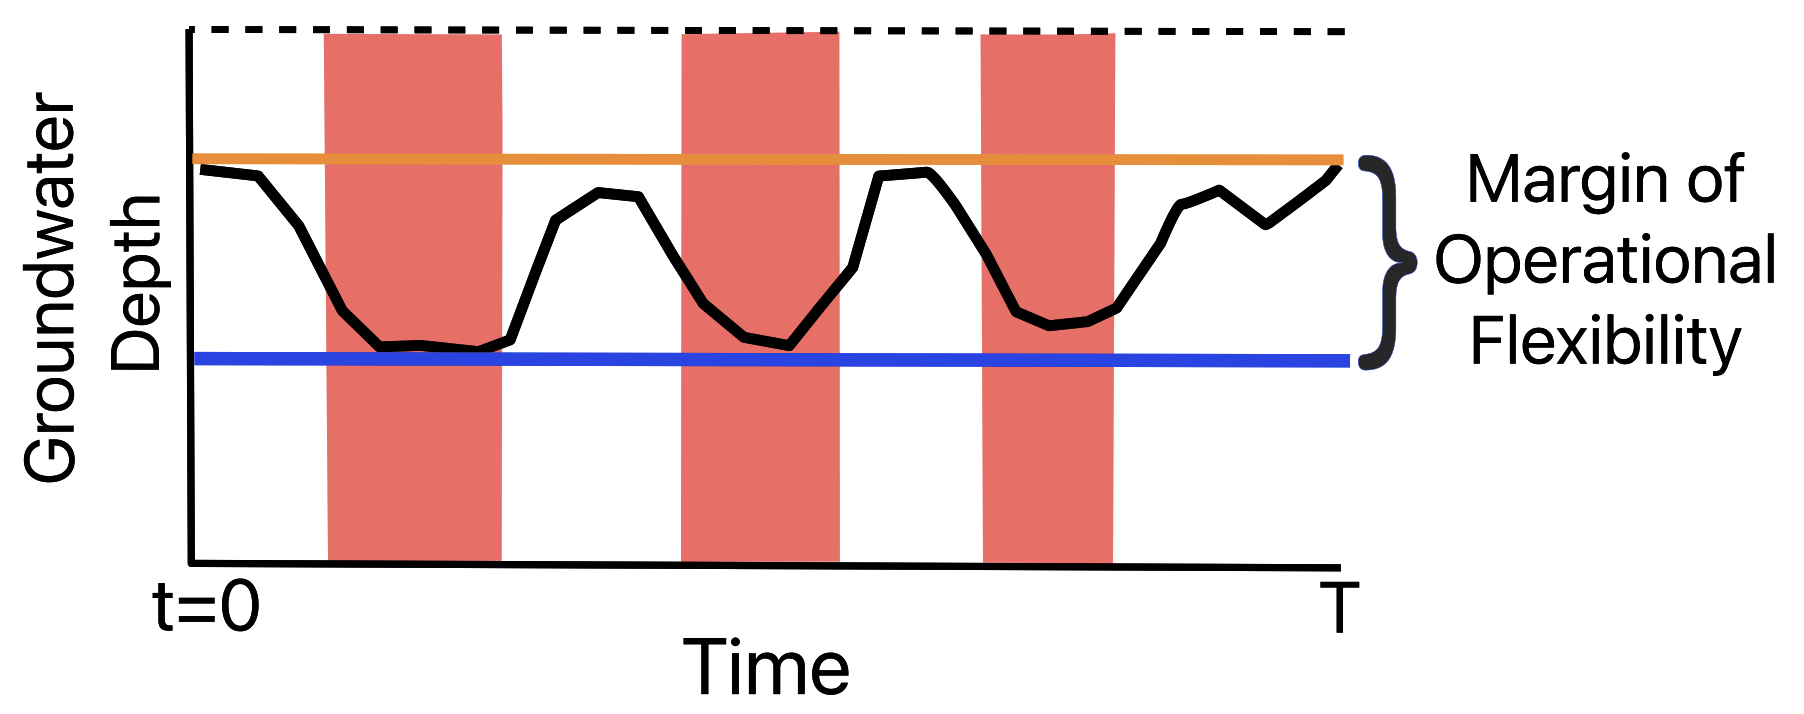
\includegraphics[width=0.7\textwidth]{conceptual_sgma_policy.jpg}
    \caption{Conceptual behaviour of groundwater depth under sustainable management. Dashed line represents the ground level, orange line depicts the measurable objective and blue line represents the minimum threshold. Red rectangles depict dry periods when groundwater depth increases.}
    \label{fig:1}
\end{figure}
  
The study area is the Semitropic Water Storage District (SWSD), located in the SJV and Kern County groundwater basin (Figure 1). The SWSD also operates its own Groundwater Sustainability Agency, which defined possible strategies that can be implemented depending on the water budget of each year. Four possible strategies are analyzed in this study: a groundwater use control and a groundwater pumping fee, implemented by the GSA, and a total land use and perennial crops planting decisions, operated by farmers. Other management strategies as water market mechanisms and supply-side policies focused on augmenting groundwater storage, as managed aquifer recharge (\cite{ulibarri_assessing_2021}), are out of the scope of this study. 

\begin{figure}[H]
    \centering
    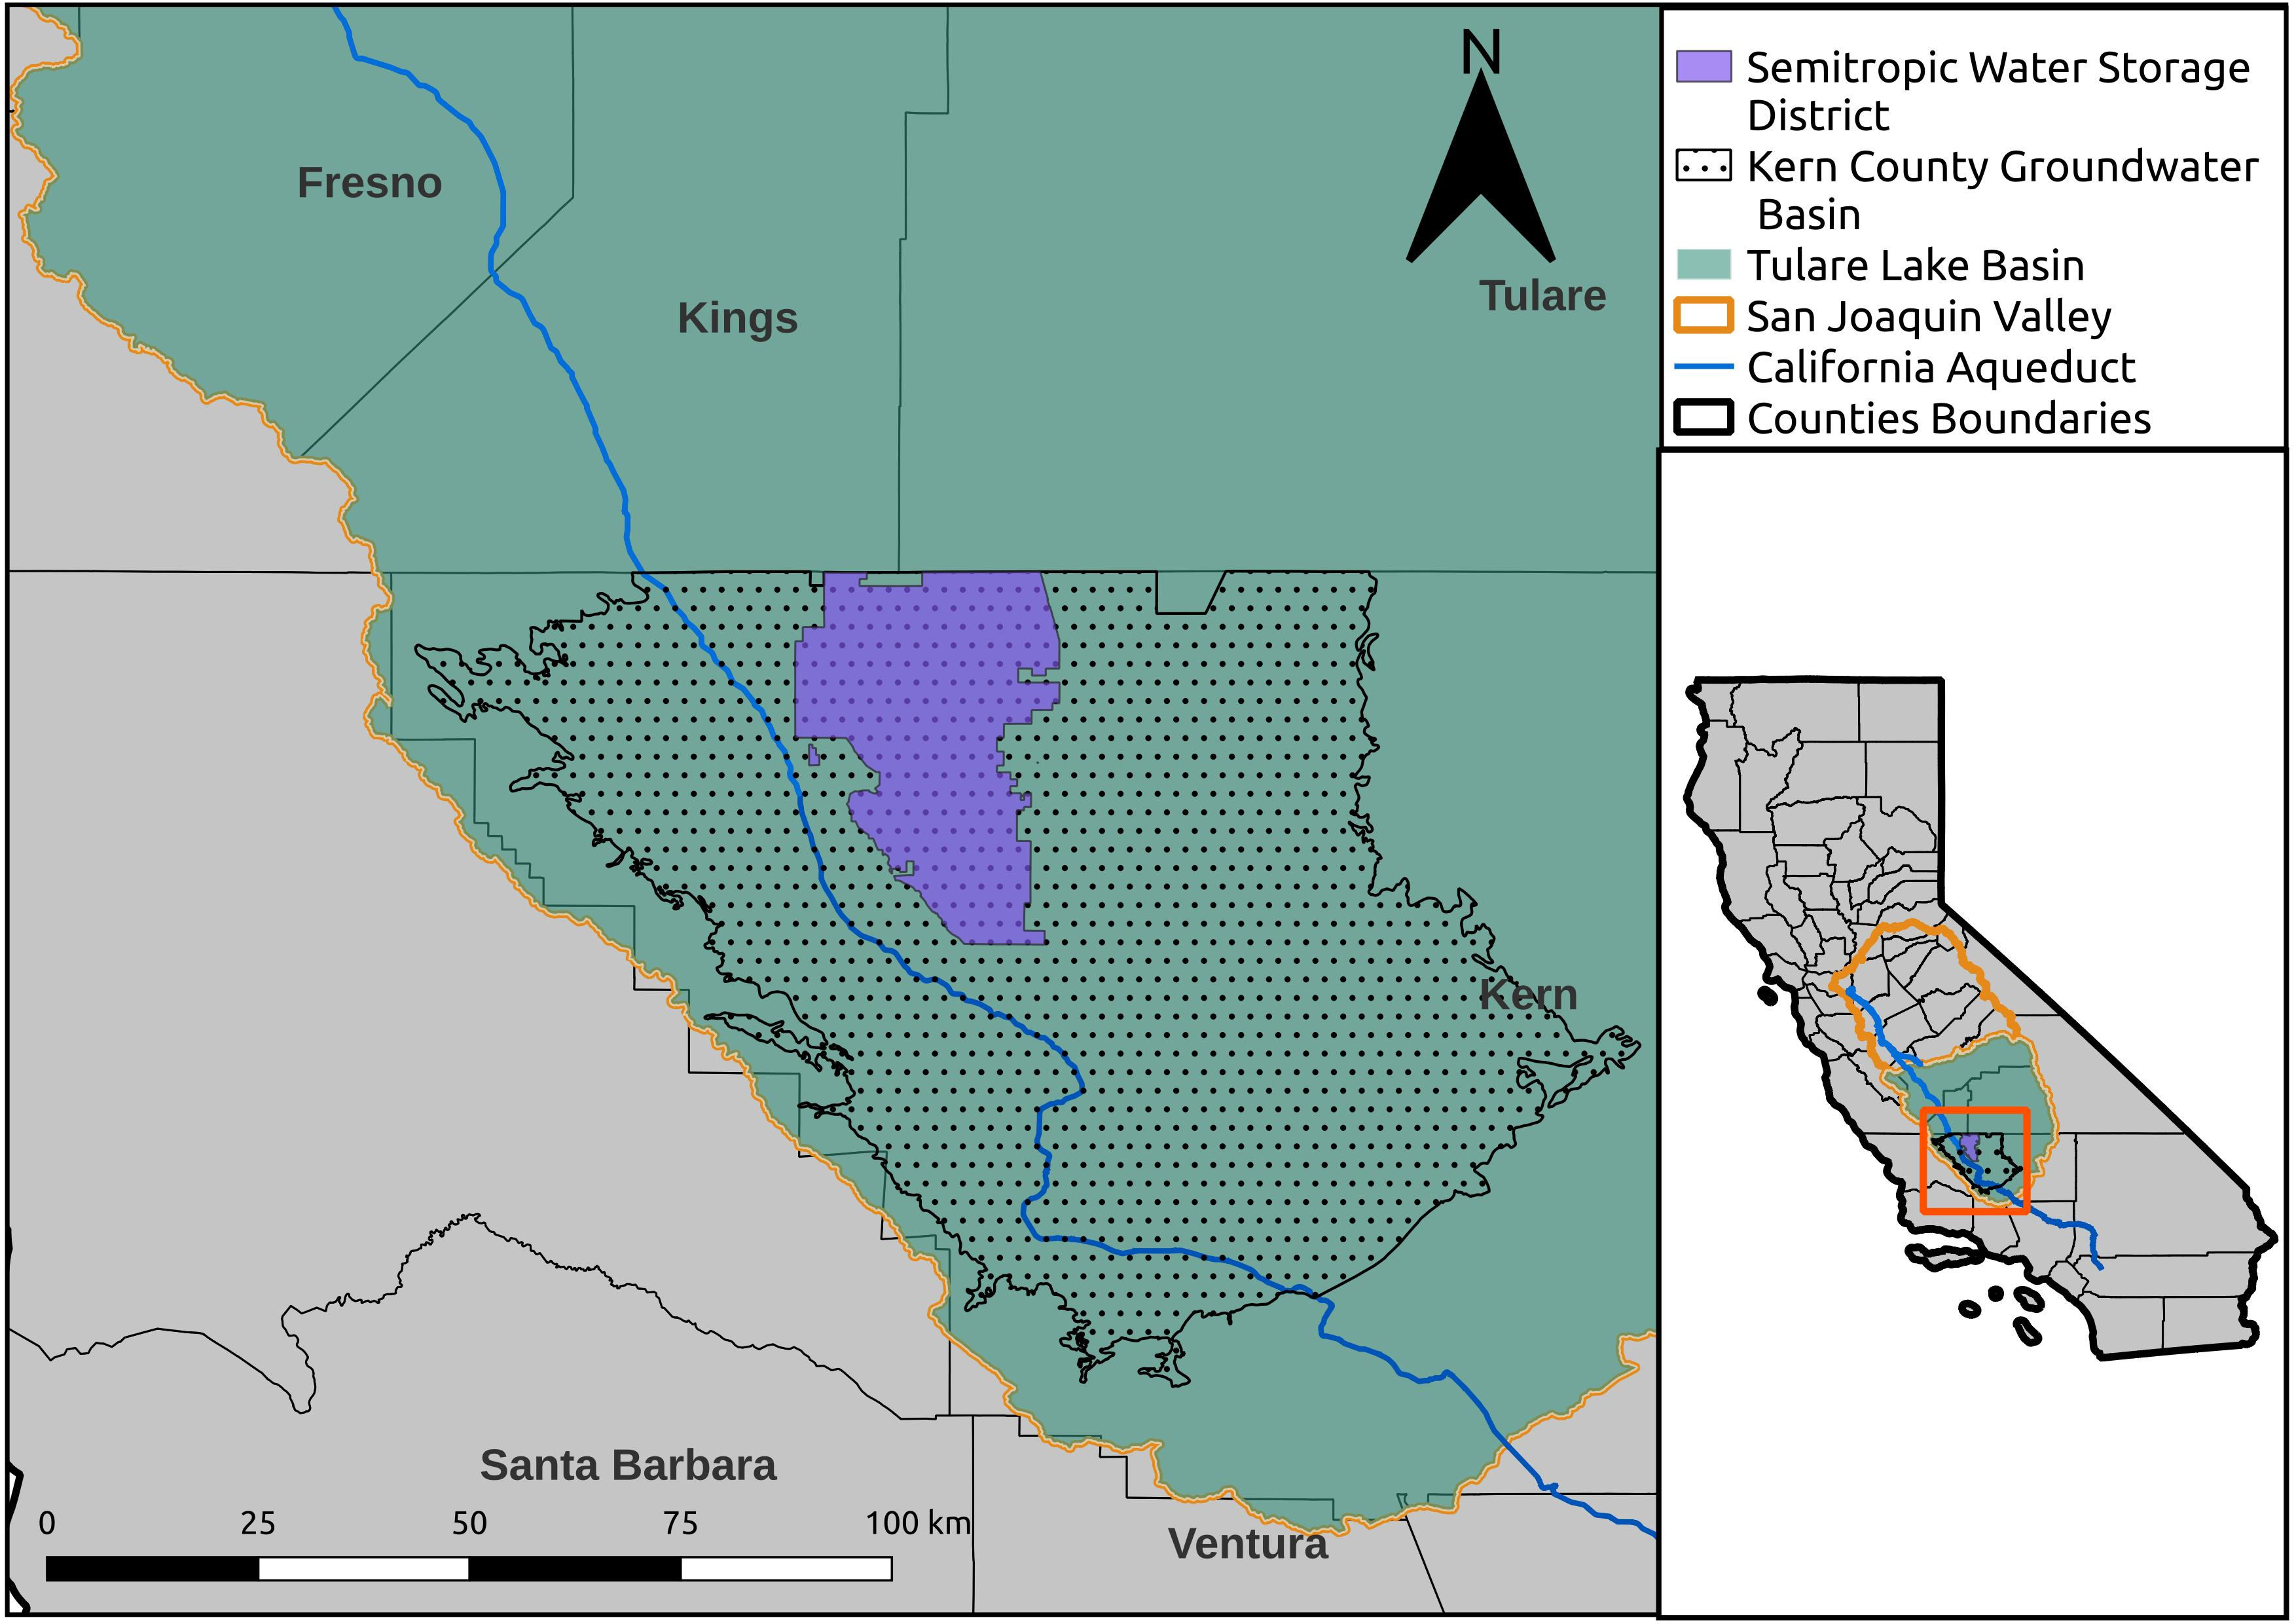
\includegraphics[width=0.8\textwidth]{Map_Semitropic.jpg}
    \caption{Semitropic Water Storage District located in the San Joaquin Valley, California}
    \label{fig:1}
\end{figure}

\section{Hydro-Economic model}

In food-water systems Hydro-Economic Models have been used as decision support modeling tools too asses water policy and climate change adaptation decisions (\cite{ward_hydroeconomic_2021,harou_hydro-economic_2009}). HEMs are able to abstract stakeholders decisions (e.g farmers) and hydrology dynamics, as well as their feedback, by integrating economic models with hydrological response functions (\cite{harou_hydro-economic_2009}). Given the modular characteristic of these coupled modeling methods is possible to assess the performance of economic revenues and aquifer dynamics, as shown by \textcite{macewan_hydroeconomic_2017}, \textcite{afshar_multi-objective_2020}, \textcite{rodriguez-flores_global_2022} and \textcite{graveline_combining_2019}. Additionally these methods are flexible to asses the performance of water management policies, under different climate scenarios, and spatial and time scales.

\subsection{Economic model}

The food production system was modeled using a hydro-economic model (\cite{harou_hydro-economic_2009}) able to represent a yearly net profit maximization at the irrigation district level. With this economic model we are able to model land and water (surface and groundwater) allocation decisions for crop production. This model assumes that farmers make production decisions to maximize revenues by taking into account crop prices, surface water availability, price of surface water, price of electricity and water management policies. We used a mathematical model based on Positive Mathematical Programming (PMP) (\cite{howitt_calibration_1995}), using a stochastic data assimilation method to calibrate the economic parameters described by \textcite{maneta_stochastic_2014} and \textcite{maneta_satellite-driven_2020}. This calibration framework enables updating the distribution of the calibration parameters every time data becomes available. See Appendix A for more information about the calibration process. 

For the calibration we used observed data from 1998 to 2015. After the last year of historical observations was Incorporated in the data assimilation process, the resultant ensemble with 400 samples of calibration parameters $\theta_{i} = [\mu_{i},\beta_{i,water},\beta_{i,land},\delta_{i},\lambda_{i,land},\lambda_{i,water},\bar{\lambda}_{land}]$ are used in the economic model. Equations 1-7 define the maximization problem.

\begin{alignat}{1}
\underset{{\substack{x_{i,land,t}\geq0\\x_{i,water,t}\geq0\\wat_{i,w,t}\geq0}}}{max}& \sum_{i} \{p_{i,t} \mu_{i}(\beta_{i,land} x^{\rho_i}_{i,land,t}+\beta_{i,water} x^{\rho_i}_{i,water,t})^{\delta_{i}/\rho_i} - (\omega_{i,land} + \lambda_{i,land} + \bar{\lambda}_{land}) x_{i,land,t} \notag \\&-(\omega_{SW,t}+ \lambda_{i,water} )wat_{i,SW,t} - (\omega_{GW,t}+ \lambda_{i,water} + u^{GWF}_{t})wat_{i,GW,t}\}
\end{alignat}

\textit{subject to}
\begin{flalign}
&\sum_{i} x_{i,land,t} \leq u^{TL}_{t}& \\
&\underset{i\in{PC}}{\sum} x_{i,land,t}  \leq  u^{PL}_{t}\\
&\underset{i\in{PC}}{\sum} x_{i,land,t}  \geq \underset{i\in{PC}}{\sum} x_{i,land_{t\mh1}} * 0.95 \\
&x_{i,water,t} = wat_{i,SW,t} + wat_{i,GW_t} \\
&\sum_{i} wat_{i,SW,t} \leq b_{SW,t}   \\
&\sum_{i} wat_{i,GW,t} \leq u^{GWP}_t \\
& x_{i,water,t} \geq \bar{x}_{i,water}*0.98
\end{flalign}

Where Equation 1 represents the revenue that is maximized by allocating land $x_{land,i}$, total water $x_{water,i}$, surface water $wat_{SW,i}$ and groundwater $wat_{GW,i}$ to each crop i (Figure A.1). $p_{i,t}$ is the price of crop $i$. Crop production in the first term of Equation 1 is represented by a CES production function (\cite{debertin_agricultural_2012}), where $\beta_{i,j=[land,water]}$ are the relative use of inputs, a scale parameter $\mu_{i}$, $\rho = (\sigma-1)/(\sigma)$ where $\sigma = 0.17$ is the elasticity of substitution parameter and $\delta_{i}$ is calibrated using the first order conditions. The rest of the parameters used in the linear costs are the calibrated Lagrange multipliers $\lambda_{water},\lambda_{land}$, associated to the observed water and land allocation per crop constraints respectively (Appendix A). Variable costs are represented by a linear cost as a function of land and water allocated, where $\omega_{i,land}$ is the cost of land, price of surface water per unit of water $\omega_{SW,t}$. The volumetric cost of groundwater pumping is given by $\omega_{GW,t}$, which is a function of price of electricity ($\omega_{E,t}$), the groundwater depth or potentiometric level ($GWD_t$) and other parameters related to the characteristics of the wells (Appendix A.2). Additionally a per cubic meter $u^{GWF}_{t}$ pumping fee can be implemented that sums to the pumping cost.

The maximization problem is subject to resources availability and land and water quantitative controls. Equation 2 is a total land restriction where $u^{TL}_{t}$ is the total land use control that can be implemented in a year $t$. Equation 3 is an upper boundary perennial crops restriction $u^{PL}_{t}$ that levers the expansion or reduction of land allocated to perennial crops, where $PC \in$ \{Almonds and Pistachios, Subtropical, Other Deciduous and Vine\}. In order to maintain the perennial crops removals to what has been observed historically we added a perennial removal constraint (Equation 4) to be no more than 5 percent of the land allocated to these crops. Equation 5 is a mass balance restriction where each crop can use water from both surface water and groundwater. Equation 6 is the Surface water availability ($b_{SW,t}$) restriction. Equation 7 is the total groundwater pumping restriction where $u^{GWP}_{t}$ is the maximum allowed groundwater pumping decision. $u^{GWF}_{t}$, $u^{TL}_{t}$, $u^{PL}_{t}$, $u^{GWP}_{t}$ are the four management decision that this study asses formulated in the adaptive control policy (Section  4). Finally we included a water stress restriction, that allows to reduced applied water to each crop category up to 5\% of the average applied water per per unit of land ($\bar{x}_{i,water}$)in the historical record.

\subsection{Groundwater Depth Response Function}

Groundwater in the San Joaquin Valley is a complex system, its dynamics depend on many geological, hydrological, climate and human components. To incorporate the dynamics of groundwater depth level (potentiometric level) we used outputs from the physical based model Fine Grid California Central Valley Groundwater-Surface Water Simulation Model (C2VSIM-FG version 1.01) (\cite{dwr_c2vsimfg_2021}) to calibrate a response function. C2VSIM-FG has a finite element grid of more than 35,000 elements for all the Central Valley California, for each element is able to link land surface, surface water and groundwater. The model uses historical data on cropland use, crop water demand, surface water diversions, precipitation, soil moisture, among others, to run its simulation process. C2VSIM-FG can be run for a simulation period from 1973 to 2015 at a monthly time step. Water budgets are generated for each element in the grid including groundwater pumping and groundwater depth and can be post-processed to create water budgets for defined boundaries (group of elements). For the purposes of this study we used the budget generated for the Semitropic Water Storage District boundary. 

From C2VSIM-FG we used the weighted-average groundwater depth level to agricultural pumping to remove the nodes where there is not agriculture within the district boundary. Since the economic model simulates farmers decisions at a yearly time step we used the groundwater depth change from the beginning of the water year (October) end of the water year and irrigation season (September), and the total groundwater pumping in a water year to calibrate the response function. Figure 2 shows the simulated groundwater depth and agricultural pumping from C2VSIM-FG at the end of the water year. 

\begin{figure}[H]
    \centering
    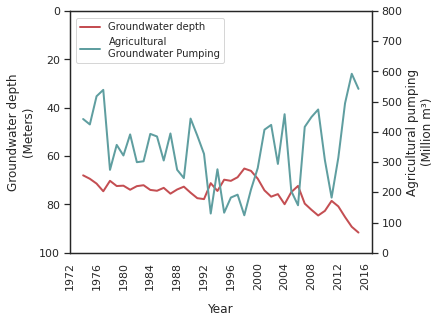
\includegraphics[width=0.5\textwidth]{c2vsim_semitropic.png}
    \caption{Groundwater depth and agricultural groundwater pumping from simulation outputs of C2VSIM-FG (\cite{dwr_c2vsimfg_2021})}
    \label{fig:mes1h1}
\end{figure}

The groundwater depth change response function was calibrated using a Bayesian linear regression (Appendix B). With this function we are able to predict at every year step the groundwater depth change as a function of total agricultural pumping. As shown by Equation 8 the ground water depth level at the beginning of the year t ($GWD_{t}$) is calculated as the sum of the groundwater depth level at the beginning of the year t-1 ($GW_{t-1}$) and the median of the predictive posterior distribution for groundwater depth change ($\overline{\Delta GWD}_{t-1}$) estimated at the end of the year t-1. By embedding this function into the economic model and by defining the pumping cost as a function of the groundwater depth (Appendix A.2) we are able to model the feed-back between food production and groundwater system.

\begin{align}
GWD_{t} = GWD_{t-1} + \overline{\Delta GWD}_{t-1}
\end{align}

\subsection{Stochastic time series}

In order to run the model dynamically we build Monte Carlo time series for economic and hydrologic conditions that feed the Hydro-economic model. Each time series starts at $t_{0}=2016$. In our analysis we included simulated surface water supplies to the irrigation district (Figure 3) from the California’s Food-Energy-Water System simulation model (CALFEWS) (\cite{zeff_californias_2021}). These were simulated with down-scaled data from seven of the ten Global Circulation Models (GCMs) suggested by \textcite{pierce_climate_2018}: CCSM4, MIROC5, CanESM2, CNRM-CM5, GFDL-CM3, HadGEM2-CC and HadGEM2-ES, and using the Representative Concentration Pathway (RCP) 4.5 (moderate scenario) and 8.5 (high emissions scenario). The surface water deliveries were scaled using the average deliveries in the historical for each GCM and RCP and the observed historical values. This study does not account on changes to crop yields and evapotransporation from climate change due to the lack of information. 

\begin{figure}[H]
    \centering
    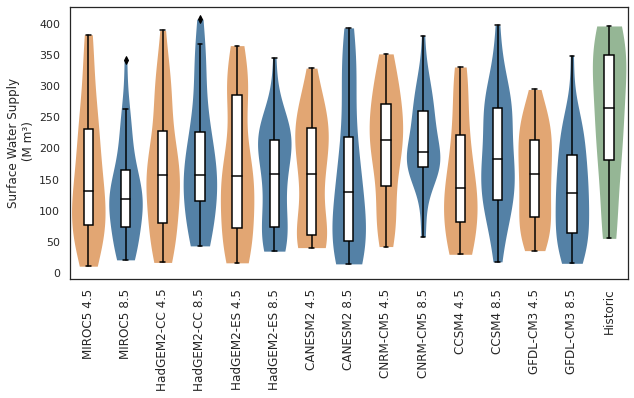
\includegraphics[width=0.7\textwidth]{gcm_surface_water.png}
    \caption{Distribution of historical (1999-2015) and projected surface water deliveries from CALFEWS (2016-2045) (\cite{zeff_californias_2021})} \label{fig:SWSemitropic}
\end{figure}

Additionally, we considered uncertainties on economical variables and calibration parameters of the PMP model, summarized in Table 1. Crop prices $p_{i,t}$ were sampled using the historical data from 1980 to 2020 (\cite{usda_national_2020}), price of electricity ($\omega_{E,t}$) was sampled from the historical (2008-2021) reported by the Pacific Gas and Electricity Company (PG\&E) for small and large agricultural users. Price of surface water ($\omega_{SW,t}$) was sampled from rates reported in different water-year types using surface water supply to define the water-year type category. Finally a sample from the posterior distribution of the calibration parameters $\theta_{i}$ is sampled.

\begin{center}
\begin{tabular}{ |c|c|c|c| } 
 \hline
 Variable & Symbol & Units & Source \\ 
 \hline
 Crop prices & $p_{i}$ & \$/ton & \textcite{usda_national_2020}\\
 Price of electricity & $\omega_{E,t}$ & $\$/Kwh$ & \textcite{pge_pacific_2021} \\
 Price of surface water & $\omega_{SW,t}$ & $\$/m^3$ & Irrigation district reports\\
 Surface water supply & $b_{SW,t}$ & $m^3$ & \textcite{zeff_californias_2021}\\
 Calibration parameters & $\theta_i$ & - & Calibration process \\
 \hline
 \end{tabular}
\captionof{table}{Data Sources for Monte Carlo Time Series}
\end{center}


\section{Adaptive Dynamic Decisions}

Searching for an adaptive groundwater management policy using DPS consist on optimizing the parameters of the control policy function that yields groundwater management decisions and their performance in the food-water system is simulated in the Hydro-economic model.  Different  parametric functions can be used to model control policies, including linear, polynomial, neural networks, decision trees and radial basis functions (\cite{giuliani_universal_2014}). In this study we used Cubic Radial Basis Functions (RBFs) to represent the complexity of the dynamic decision making in the irrigation district where every year the GSA can coordinate different management decisions given surface water supply, crop-land decisions, and groundwater depth at the beginning of the irrigation season. The four decisions in the control policy analyzed in this study are: Groundwater pumping fee (GWF), total land restriction (TL), perennial cropland restriction (PL) and groundwater pumping restriction (GWP). 



\subsection{Direct Policy Search}

Dynamic land and groundwater management decisions made at every year step $t$ are represented by the vector $u_{t}^D$ where $D \in \{GWP,TL,PL,GWF\}$ represent the four possible decisions. The control policy in Equation 10 equals to the outputs of a policy $P^D$ which is a mathematical function with two vector inputs: the structural parameters of the RBFs ($\psi^D$) and system-state information vector ($I_{t'}$). Information variables in $I_{t'}$ represent key components of the food-water system which values can be from the current year $t$ or previous year $t-1$. 

\begin{align}
u_{t}^D = P^{D}(I_{t'}|\psi^{D})
\end{align}

In direct policy search, the use of RBFs have shown to be an efficient way to represent complex decision making. These have been applied to lake pollution control (\cite{quinn_direct_2017}), reservoir operation (\cite{giuliani_universal_2014, zatarain_salazar_balancing_2017}), sea-level rise protection (\cite{garner_using_2018}), and financial risk management in water-energy systems (\cite{gupta_can_2020,hamilton_stream_2022}). For this study we define the control policy function $P^D$ as set of cubic radial basis functions given by Equation 10.

\begin{align}
u_{t}^D = \phi^{D}\left(\sum_{m=1}^M w_{m}^D \sum_{j=1}^J \left\lvert\dfrac{[I_{t'}]_{j}-c_{j,m}}{r_{j,m}}\right\rvert^{3}\right)
\end{align}

Where $\phi^{D}$ is an outer function, $w_{m}^D$ is the weight of M cubic radial basis functions. The weights can have values $ 0 \leq w_{m} \leq 1$ and are subject to $\sum_{m=1}^M m_{m}^D= 1$. The four decisions in the control policy share the same RBFs structure; hence the information vector $I_{t'}$ is shared for all decisions. $I_{t'}$ in Equation 12 is a vector with system state variables that inform the policies, where $\overline{GWD}_{t}$ is the normalized level to groundwater at the beginning of the year, $\overline{PCL}_{t-1}$ is the normalized area devoted for perennial crops production in the year $t-1$. $\overline{b}_{SW,t}$ is the normalized surface water available in year $t$. Normalization was performed using $k^{GWD}$, $k^{TL}$, $k^{SW}$ to obtain $\overline{GWD}_{t}$, $\overline{PCL}_{t-1}$, $\overline{b}_{SW,t}$ respectively summarized in Table 2. Additionally, $c_{j,m} \in [-1,1]$ and $r_{j,m} \in (0,1]$ are the center and radius respectively shared by all the RBFs.

\begin{align}
I_{t'} = [\overline{GWD}_{t},\overline{PCL}_{t-1},\overline{b}_{SW,t}]
\end{align}

The function $\phi^{D}$ in Equation 10 can consist on two functions, unnormalize $\phi^{D,N}$ and constraint $\phi^{D,C}$, used to obtain the values of the management decisions in the control policy $u_{t}^D$. Being $z_{t}$ the argument in the $\phi^{D}$ function (Equation 11), the value of each decision is defined by the following equation.

\begin{align}
u^{D}_t = \phi^{D,C}(\phi^{D,N}(z_{t}))
\end{align}

For the groundwater pumping restriction policy ($u^{GWP}_t$) $\phi^{GWP,N}$ scales the groundwater that farmer will have available to pump between zero and the pumping capacity of the district $k^{GWP}$ (maximum observed pumping). $\phi^{GWP,C}$ constraints the groundwater pumping to be at least the difference between the water demand by perennial crops of the year $t-1$ and the surface water available in the year $t$. 

\begin{align}
z'_{t}=\phi^{GWP,N}(z_{t}) = k^{GWP}max(min(z_{t},1),0) 
\end{align}

\begin{align}
u^{GWP}_t = \phi^{GWP,C}(z'_{t})= max(z'_{t},\underset{i \in PCL}{\sum} x_{i,water_{t\mh1}} - \; b_{SW,t})
\end{align}

In Equation 16 the unnormalize function ($\phi^{TL,N}$) scales the total land decision that farmers can produce in the district for the year t, between zero and $k^{TL}$, where $k^{LR}$ is the total land in the district (maximum observed produced land). As shown in Equation 15, $\phi^{TL,C}$ constraints the total land decision to be at least the land used by perennial crops in the the year $t-1$.

\begin{align}
z'_{t} = \phi^{TL,N}(z_{t}) = k^{TL}max(min(z_{t},1),0)
\end{align}

\begin{align}
u^{TL}_t = \phi^{TL,C}(z'_{t})= max(z'_{t},\underset{i \in PC}{\sum} x_{i,land_{t\mh1}})
\end{align}


For the perennial crops planting restriction ($u^{PL}_t$), $\phi^{PL,N}$ scales the total land that can be allocated to perennial crops between zero and the total land available in the district ($k^{TL}$). $\phi^{PL,C}$ constraints the perennial restriction to be at least 95\% of the previous year perennial crops land, and it limits the expansion of perennial crops to 5\% more acreage from the previous year $t-1$. These restrictions are applied to ensure that solutions of the control policy are realistic to what has been observed the region.

\begin{align}
z'_{t} = \phi^{PL,N}(z_{t}) = k^{TL}max(min(z_{t},1),0)
\end{align}

\begin{align}
u^{PL}_t = \phi^{PL,C}(z'_{t})= \begin{cases}
      \underset{i\in{PC}}{\sum} x_{i,land_{t\mh1}}*1.05,  \text{\; if \, $z'_{t}$  $>$ $\underset{i\in PC}{\sum}x_{i,land_{t\mh1}}*1.05$}\\
       \underset{i\in PC}{\sum} x_{i,land_{t\mh1}}*0.95, \text{\; elif \, $z'_{t}$  $<$ $\underset{i\in PC}{\sum}x_{i,land_{t\mh1}}*0.95$}\\
      z'_{t}, \text{\; $otherwise$}
\end{cases}     
\end{align}

Finally for the pumping fee ($u^{GWF}_t$), the function $\phi^{GWF}$ in Equation 20, scales the groundwater pumping fee that can have values between [0,$k^{GWF}$]. $k^{GWF}$ is set to be $\$0.4/m^3$, hence the upper boundary of the pumping fee is 0.4 USD per cubic meter. This fee sums to the groundwater pumping cost in the objective function of the economic model (Equation 1).

\begin{align}
u^{GWF}_t = \phi^{GWF,N}(z_{t}) = k^{GWF}max(min(z_{t},1),0)
\end{align}

The dynamic control policy is represented by the set of Equations 11 to 20, where the vector of structural parameters $\psi = [w^{D},c,r]$ is optimized. Since the information vector $I_{t'}$ of size $J$ is shared across decisions in $M$ number of RBF's the vectors of centers (c) and radii (r) are equal to $c=[c_{0,0},...,c_{J,M}]$ and $r=[r_{0,0},...,r_{J,M}]$.


\begin{center}
\begin{tabular}{ |c|c|c|c| } 
 \hline
 Variable & Symbol & Units & Value \\ 
 \hline
 Normalization for cropland  & $k^{TL}$ & $Kha$ & 62\\
 Normalization for groundwater pumping & $k^{GW}$ & $M m^3$ & 732 \\
 Normalization groundwater depth  & $k^{GWD}$ & $m$ & 198 \\
 Normalization for pumping fee   & $k^{GWF}$ & \$/$m^3$ & 0.49 \\
 Normalization surface water  & $k^{SW}$ & $M m^3$ & 208 \\
 \hline
 \end{tabular}
\captionof{table}{Normalization factors used in the control policy}
\end{center}


\subsection{Bi-level Optimization Problem}

This study implements two optimization processes (Figure 5). A MOEA is performed that optimize the vector of structural parameters in the RBFs ($\Psi$). Each set of structural parameters define a control policy or set of decisions ($u^{D}$) which are assessed in the Hydro-economic model using N Monte Carlo realizations with times series of T years. We let the Hydro-economic model find optimal land and water allocation for the first five years of each time series resolution, hence at t=5 the model starts the implementation of management decisions and the assessment of objectives. This was done to simulate the path towards sustainability described in Section 2.1 and Figure Sx. The results of the  process are aggregated in five performance metrics, representing the groundwater sustainability and economic goals of the irrigation district. These objectives feedback to the MOEA to continue its optimization process. 

\begin{figure}[H]
    \centering
    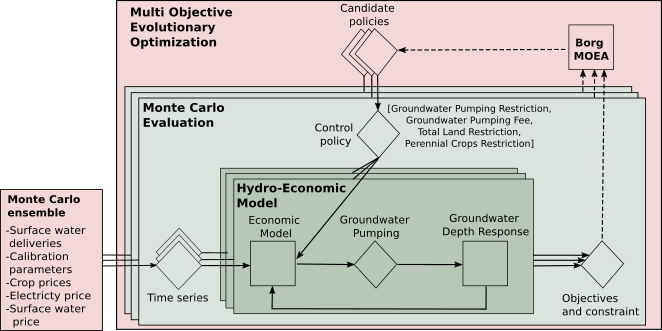
\includegraphics[width=0.9\textwidth]{Diagram2}
    \caption{Bi-level optimization problem schematic adapted from \textcite{hamilton_stream_2022}. Rectangles represent the modules that contain optimization and simulation models (squares) and inputs/outputs (diamonds). Dashed arrows depict the Borg MOEA feed-back process where the values of objectives and constraint are from performance metrics of the Hydro-economic model result of an implemented control policy.}
    \label{fig:m1esh1}
\end{figure}

The first level optimization consists in a multi-objective evolutionary optimization where five objectives are minimized or maximized, the decision variables are the structural parameters of the RBFs in the vector $\Psi$, used to parameterize the control policy. 

\begin{align}
\underset{\Psi}{argmin} = (-O_{1}(\Psi),O_{2}(\Psi),-O_{3}(\Psi),O_{4}(\Psi),-O_{5}(\Psi))
\end{align}

The first objective ($O_{1}$) is to to maximize the average total revenues $\pi_{n,t}$ from the total net revenue of N ensemble realizations with T years. This objective represents the economic objective of farmers of revenue maximization. A lower boundary constraint for this objective is defined to achieve at least an average total revenue greater or equal than \$11 billions. This restriction constraints the algorithms from finding unrealistic policies and far from farmers preferences. 

\begin{align}
O_{1} = \frac{1}{N}\sum_{n=1}^N(\sum_{t=5}^T \pi_{n,t})
\end{align}


\begin{align}
O_{1} \geq 11,000
\end{align}

The second objective is the minimization of the average groundwater depth. The average of groundwater depths is taken over the T years for each Monte Carlo realization, and then the average of these are taken over all the N Monte Carlo realizations. 

\begin{align}
O_{2} = \frac{1}{N}\sum_{n=1}^N(\frac{1}{T}\sum_{t=5}^T GWD_{n,t})
\end{align}

The third objective is to minimize the 5th percentile of minimum profits. This metric represents a \textit{max-min} goal, used to inform decision makers about the of the worst profits in a given year. Even though, there are economic factors included in the stochastic ensemble that can be drivers of low economic revenues, management decisions can be the main causes of expected low profits particularly during dry years, as shown by \textcite{rodriguez-flores_global_2022}. 

\begin{align}
O_{3} = Q5_{N} \bigg[\underset{t\in(5,...,T)}{min}[\pi_{n,t}]\bigg]
\end{align}

The fourth objective is to minimize the 95th percentile of maximum groundwater depths. This objective represents a \textit{min-max} goal of the largest groundwater depth.  The maximum groundwater depth level is taken over each ensemble of T years and the Q95 operator takes the 95th percentile over all N the Monte Carlo  realizations. 

\begin{align}
O_{4} = Q95_{N} \bigg[\underset{t\in(5,...,T)}{max}[\overline{\Delta GWD}_{t-1}]\bigg]
\end{align}

As explained in Section 2.1 during dry years the distance to groundwater can go bellow the measurable objective, expecting that in wet years it will recover. However, the objective is to maximize the number of years that the groundwater depth is at the measurable objective level (or lower) limiting the groundwater level to go above the minimum threshold. Thus, the fifth objective is to maximize the average fraction of years (reliability) that the distance to the groundwater depth is above or at the measurable objective ($GWD^{SGMA}$).  We used the 2015 groundwater level from C2VSim-FG as measurable objective. Additionally we included a constraint (Equation 27) that the reliability has to be at least 20\% (i.e. one of every five years). 

\begin{align}
O_{5} = \frac{1}{NT}\sum_{n=1}^N(\sum_{t=5}^T-5 \tau_{n,t})\; where\; \tau_{n,t} = \begin{cases}
      1, \text{\; $GWD_{n,t}$  $\leq$ $GWD^{SGMA}$}\\
      0, \text{\; $GWD_{n,t}$ $>$ $GWD^{SGMA}$}\\
\end{cases}      
\end{align}


\begin{align}
O_{5} \geq 0.2
\end{align}

\subsection{Robustness Analysis}

Solutions in the Pareto front are heterogeneous control policies with different levels of trade-offs among objectives from which stakeholders can visualize their preferences and find acceptable policies. However, given the large number of results might be hard to understand and summarize the performance of the policies across multiple states of the world (\cite{herman_how_2015}). Robustness analysis commonly used in robust decision making frameworks (\cite{marchau_decision_2019}), can help to select policies based on stakeholders preferences or constraints on expected performance of the system (\cite{kasprzyk_many_2013}). Different metrics can be used to measure the robustness of each control policy representing different farmers and water managers acceptability thresholds and their perception of risk (\cite{mcphail_robustness_2018}), filtering the solutions. For this study we selected the domain criterion satisfying metric (\cite{schneller_decision_1983}) that quantifies the fraction of scenarios that achieve the minimum performance by stakeholders. 



\section{Computational Experiment}

The search of optimal RBFs parameters in EMODPS is a non-convex problem (\cite{giuliani_curses_2016}) that can be solved using heuristic methods. MOEAs are stochastic search tools that perform an iterative process using evolutionary strategies inspired from nature to evolve and to improve a population of possible solutions that optimizes multiple objectives. This process is done until a population reach a Pareto front or non-dominated solutions (\cite{coello_evolutionary_2007}), while running the hydro-economic model dynamically. 

\subsection{Experiment Algorithms}  

For this study we use the Borg MOEA (\cite{hadka_borg_2013}), a self adaptive algorithm that uses probabilistic operators as $\epsilon$-dominance, adaptive population sizing and time continuation through $\epsilon$-progress. Borg MOEA has shown have better time efficiency, scalability and controllability, as well as less sensitive to its parameterizations compared to other MOEA algorithms (\cite{reed_evolutionary_2013}).  These characteristics and its support to different parallelization variants makes it widely applicable to complex problems with different scales and computational demands (\cite{hadka_large-scale_2015}). Since Borg MOEA is a stochastic algorithm we estimate Pareto-front solutions using ten different random seeds using the master-worker parallel configuration of Borg (\cite{hadka_large-scale_2015}). $\epsilon$-values (resolution) for each objective and the Borg MOEA parameter values are summarized in SI Table S2 and S3. 

The economic model (Equations 1-7) was formulated using the Python package Pyomo (\cite{hart_pyomo_2011}) and solved using the non-linear programming solver IPOPT (\cite{wachter_implementation_2006}). The decision variables in the economic model are the allocation of land and water (surface water and groundwater) to seventeen crop groups resulting in 68 decision variables by each time step $t$. Additionally at each time step a posterior predictive sample of groundwater depth change with 400 samples was estimated using the model and trace generated using the probabilistic programming Python package PyMC  (\cite{salvatier_probabilistic_2016}).

We performed the bi-level optimization process for an ensemble of N = 100 Monte Carlo realizations and T = 30 years for 50,000 candidate policy trials (function evaluations). A structure of M=4 RBFs (Equation 11) was selected given its good performance, resulting in 40 decision variables in the vector $\Psi$ to be optimized with Borg MOEA. The final pareto-set solutions were selected from the random seed with the highest hypervolume (\cite{hadka_large-scale_2015}), shown in the Figure S4 (SI 5). The selected Pareto-set was later assessed in a larger set of Monte Carlo ensemble of N = 400 to inform the robustness analysis. All the computational experiments were performed in the MERCED cluster of the University of California Merced. 


\section{Results and Discussion}

Figure 5 shows the selected approximate Pareto-front that spans different trade-offs among the five objectives in the problem. In the figure each triangle represents a different control policy ($\Psi$ values). The star represents the ideal solution where the average groundwater depth is closer to the ground levels and farmers achieve the highest possible revenue across the sustainable management implementation period. Given the trade-offs between revenues and groundwater sustainability as the average groundwater depth decreases economic revenues decrease. We can observe that average groundwater depth decreases as reliability increases, however as the policies reach one hundred percent of reliability these rely on limiting the pumping that agriculture is using, including dry years, resulting in lower revenues. These solutions represent decisions that are unlikely to be applied in the water district as achieving the measurable objective all the years is not the objectives of a flexible management. The size of the triangle depicts the 95th percentile of the maximum groundwater depth change in a year, and the color gradient depicts the 5th percentile of the minimum revenue in a year. 

\begin{figure}[H]
    \centering
    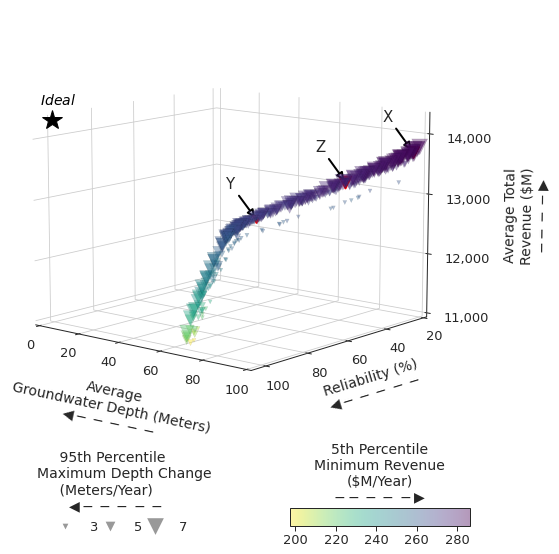
\includegraphics[width=0.8\textwidth]{selected_policies_3d.png}
    \caption{Pareto approximate set from the EMODPS experiment} \label{fig:parallel_robustness}
\end{figure}

To assess the adaptive capacity of the resultant policies to uncertain future system conditions, underscoring uncertain surface water supplies, we selected three policies that achieve different levels of reliability. Y, Z and X represent policies different trade-offs summarized in Table 3. These control policies were used to run the dynamic formulation of the control policy with four management decisions that can be taken every year before the irrigation season starts, for a 30 year time series resolution from the Monte Carlo ensemble. We selected a state of the world with the largest standard deviation on surface water deliveries (CANESM2 8.5) due to its good representation of the region characteristics with dry periods with wet years in between. As in the experiment we let the model to run five years with no management policies starting the implementation of decisions at t=5.

\begin{center}
\begin{tabular}{ |c|c|c|c|c|c| }
 \hline
 Solution & O1 & O2 & O3 & O4 & O5 \\ 
 \hline
X &  13,718 & 98.14 &  285 & 4.9 & 22\% \\
Y &  13,053 & 87 & 267 & 3.6 & 90\% \\
Z &  13,381 & 91.7  & 277 & 5.3 & 50\% \\
\hline
\end{tabular}
\captionof{table}{Performance of the selected policies shown in Figure 5}
\end{center}

Figure 6, shows the evolution of the dynamic management decisions and their performance in the food-water system. Before the management policies were implemented perennial cropland expanded relying on pumping due to reduced surface water, augmenting the groundwater depth. At the time of implementation we can observe how the decisions (Sub-figures (b) to (e)) evolve, showing the adaptive dynamic performance of the control policy. The total land planting decision, shown in Sub Figure (e), is the only decision that showed a not implementation behaviour, given that other decisions regulate land use via groundwater pumping that result in a better performance of the system. In general, we can observe similar behaviour across the other three decisions in the selected control policies, however depending on where the solution is located in the approximate Pareto-set the magnitude of the decisions change. The three solutions show that during dry years and at early stages of management a groundwater restriction should be implemented. Additionally, policies show a declining land allocation to perennial crops by 40\%. This shows that sustainable groundwater management benefits from reducing inflexible water demand from perennial tree crops as suggested by \textcite{qin_flexibility_2019}. 

During dry years control policies allow pumping to off-set lack of surface water, however these do not reach the pumping capacity and rather limit pumping to be extracted at a threshold, which can be considered a safe yield as shown by \textcite{miro_framework_2019} and \cite{macewan_hydroeconomic_2017}. We can observe that after t=10, when perennial tree crops have been reduced by the perennial planting decision, the control policy regulates most of the planting via groundwater pumping fee (Sub-Figure 6 (c)). Control policies implement a pumping fee for all the implementation period, however this augments during wet years to limit the expansion of annual crops and maximize groundwater recovery. Implementing a pumping fee can improve the irrigation efficiency and controls the expansion of cropland during wet and dry years as suggested by \textcite{stone_economic_2022}, \textcite{graveline_combining_2019}, and \textcite{khan_effect_2019}. Additionally, control policies manage annual crops planting (Sub-Figure (j)) to work as a flexible land use where at the beginning of implementation these crops reach its lowest level to allow a rebound of the groundwater level and after that they are regulated in a flexible way through the use of groundwater between wet and dry years. 

\begin{figure}[H]
    \centering
    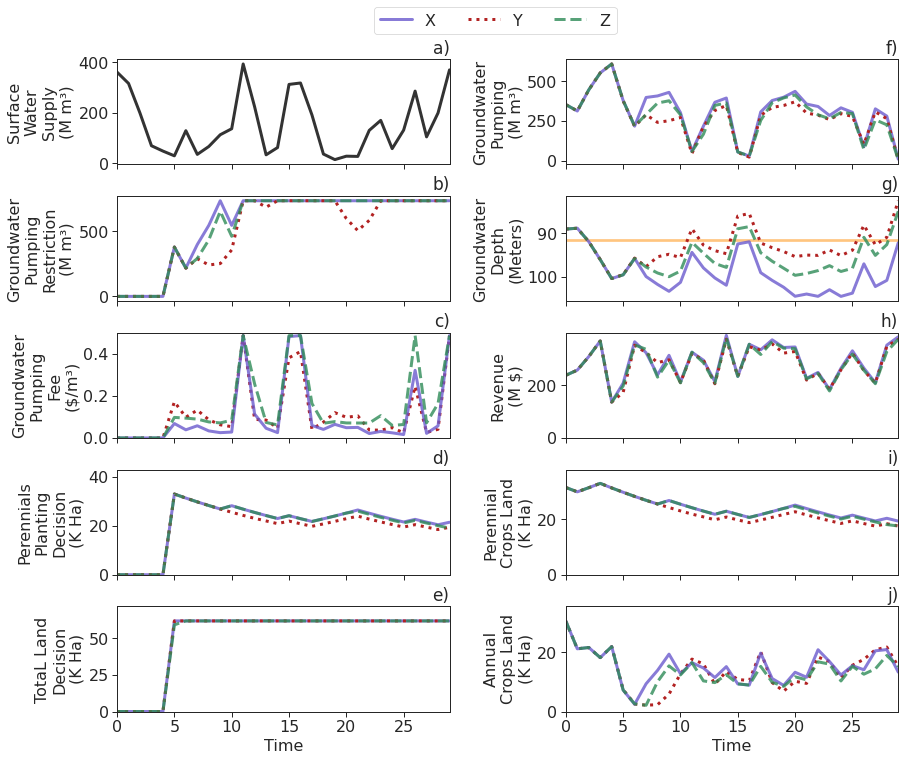
\includegraphics[width=1\textwidth]{selected_policies_performance.png}
    \caption{Performance of the dynamic policies and hydro-economic model over a 30 year realization period with 25 five years implementation of land and groundwater management decisions. Sub-figure (a) shows the surface water deliveries.Sub-figures (b) to (e) show the dynamic decisions in the control policy. Sub-figures (f) to (j) show the performance of the food-water system. The orange line in Sub-figure (g) depicts the measurable objective used in the experiment} \label{fig:parallel_robustness}
\end{figure}

Selecting different solutions along the Pareto approximate set enable us to asses their performance and provide insight of potential trade-offs of implementing management decisions. As shown in Sub-Figure 6 (g) implementing the control policy Y results in a lower average groundwater depth and larger number of years where the "measurable objective" is met. However, solutions X and Z achieved the measurable objective in wet years and also allowed having higher cropland than solution Y. 
We can observe that the control policies stopped the decline in groundwater depth observed in the historical (Figure 2), allowing the groundwater depth to reach a level where it can recover during wet years and be able to meet the "measurable objective". This behaviour is similar to what the state's management criteria suggest with the "minimum threshold", however as shown by the results it will only feasible to maintain the groundwater depth within the margin of operational flexibility if land and water management is flexible enough and the rate of years that the groundwater depth reaches the measurable objective will also depend on the capacity to limit pumping during dry years and maximize recovery in wet years. If these conditions are not met policies may fail to stop the  as observed in previous droughts and the ongoing drought that started in 2020, shown by \textcite{liu_groundwater_2022}.

\subsection{Robustness Analysis}

As we saw different policies can result in different system performances, and selecting policies for further exploration can be difficult given the large set of solutions. How ever by using the domain criterion satisfying measure we could reduce the solution space and focused on policies that meet desirable minimum criteria that the GSA and farmers can define under potential future scenarios. For this study we used the define an example of performance criteria and rates of success defined in Table 4 that a policy need to achieve to be consired robust.  


\begin{center}
\begin{tabular}{ |c|c|c| }
 \hline
 Variable Description & Threshold Value & Rate of Success \\ 
 \hline
Minimum Revenue in a year   (M USD/year)  & > 270 & > 70\% \\
Minimum Total Revenue  (M USD)  & > 12,500 & > 80\% \\
Minimum Groundwater Depth in a Year (m/year)  & < 91.4 & > 20\%  \\
Maximum Groundwater Depth in a Year (m/year)  & < 115 & > 99\%  \\
Minimum Perennial Trees Land in a year (hectares/year)  & > 50\% baseline & > 90\%  \\
\hline
\end{tabular}
\captionof{table}{Criteria for selection of Robust policies}
\end{center}

Following this criteria we found that only twelve out four hundred twenty six solutions met the performance criteria and rate of success. The performance of these polices can be explored, as we did for two robust policies(Figure 8). The one with the largest total average revenue and the one with the lowest average groundwater depth using the 400 Monte Carlo resolutions. Results can be found in SI 7, from assessing their performance using the surface water deliveries with highest standard deviation, lowest average deliveries and largest average deliveries. 

\begin{figure}[H]
    \centering
    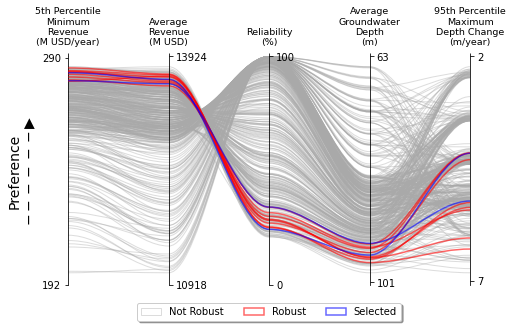
\includegraphics[width=0.7\textwidth]{robust_policies_parallel_axis.png}
    \caption{Policies from Pareto approximate set shown Figure 6. Robust Policies are in red and selected robust policies in blue.} \label{fig:parallel_robustness}
\end{figure}

\subsection{Limitations and Future Work}

Salinity other mechanisms possible expansion of water supplies 

\section{Conclusions}

\section*{Acknowledgements}

This work was supported by the NSF INFEWS program grant number 1639268 (P.I. Charaklis). José M. Rodríguez-Flores was partially supported by the UC Mexus-CONACYT scholarship. This research was conducted using MERCED cluster (NSF-MRI, \#1429783) at the Cyberinfrastructure and Research Technologies (CIRT) from the University of California Merced. We acknowledge the support from students from the Water Systems Management Lab at UC Merced who supported with data collection Spencer A. Cole, Elisa Gonzales and Kimberly Parra. VIC-CropSyst results used to estimate the crop yield elasticity to water were provided by Tina Karimi. The model C2VSim-FG outputs were provided by Jorge A. Valero Fandiño. The views expressed in this work represent those of the authors and do not necessarily reflect the views or policies of the Semitropic WSD or the California Department of Water Resources.

\section*{Data Availability Statement}

To access the Python code used for the computational experiment and  visualization of the results readers can refer to the Github repository: \url{https://github.com/josemrodriguezf/EMODPS_SGMA}.

\newpage
\appendix
\renewcommand\thefigure{\thesection.\arabic{figure}} 
\setcounter{figure}{0}  
\renewcommand{\theequation}{\thesection.\arabic{equation}}\
\setcounter{equation}{0} 
\renewcommand{\thetable}{\thesection.\arabic{table}}\
\setcounter{table}{0} 

\section{Appendix A: Economic Model Calibration}

We used a Positive Mathematic Programing (PMP) calibration that uses a stochastic data assimilation process to calibrate the economic model (\cite{maneta_satellite-driven_2020}).  With this calibration we address two objectives: avoid the assumption that farmers will behave as a particular year or average of years but rather capturing the mid-term farmers behaviour using all the data available from 1999 to 2015, and second we account for the uncertainty in the calibration parameters inherited from uncertain inputs and observations used in the calibration. This stochastic framework enables to update the distribution of parameters as new observations become available. We adapted the Python code used by \textcite{maneta_satellite-driven_2020} that performs a Monte Carlo recursive Bayesian estimator based on the ensemble Kalman Filter (enKF) (\cite{evensen_sequential_1994}). The enKF uses uses the calibration conditions to recursively update the distribution of the parameters using historical data on crop production, land use, water use, own-price supply elasticities, crop yield response to water (elasticity) and production costs. The optimally conditions to perform the stochastic assimilation are following the PMP calibration described by \cite{merel_fully_2011}, which uses using a generalize Constant Elasticity of Substitution (CES) production function as a convex production function and the calibration of the Lagrange multipliers used in the linear costs of land and water explained by \textcite{garnache_calibration_2017}. 

The goal of the calibration is to replicate observed inputs allocation to crops and yield. Following the necessary and sufficient optimality conditions or Karush-Kuhn-Tucker conditions of the maximization problem (Equations A.1) that are solved so the model calibration parameters are able to reproduce the observed allocation of inputs land and water per crop ($\tilde{x}_{i,land},\tilde{x}_{i,water}$).

\begin{flalign}
&\underset{{\substack{x_{i,land}\geq0\\x_{i,water}\geq0}}}{max} \sum_{i} \{p_{i}\mu_{i}(\beta_{i,land} x^{\rho_i}_{i,land}+\beta_{i,water} x^{\rho_i}_{i,water})^{\delta_{i}/\rho_i} - (\omega_{i,land}) x_{i,land}-(\omega_{i,water})x_{i,water}\}&\notag
\end{flalign}
\textit{subject to:}
\begin{flalign}
&\sum_{i} x_{i,land} \leq b_{land}[\bar{\lambda}_{land}]&\\
&x_{i,land} = \tilde{x}_{i,land}[\lambda_{i,land}]\notag\\
&x_{i,water} = \tilde{x}_{i,water}[\lambda_{i,water}]\notag
\end{flalign}

Where $\mu_{i},\beta_{i,water},\beta_{i,land},\delta_{i},\rho_i$ are the calibration parameters used in Constant Elasticity of Substitution (CES) production function (\cite{merel_fully_2011}) and $\lambda_{i,land},\lambda_{i,water},\bar{\lambda}_{land}$ the Lagrange multipliers for the total land and crop-specific use of inputs restrictions. The crop-specific input use restriction guarantee that the solution will reproduce the observed. $p_i$ is the crop price per crop and $\omega_{i,land}$ and $\omega_{i,water}$ the costs of land and water (weighted cost of surface water and groundwater) respectively. Even though the economic model described in Section 3.1 solves for two sources of water (groundwater and surface water), the calibration was performed aggregating both sources of water. Calibration parameters and crop specific Lagrange multipliers are obtained for the crop groups $i\in$ \{Alfalfa, Almonds and Pistachios, Corn, Cotton, Cucurbits, Dry Beans, Fresh Tomatoes, Grain, Onions and Gralic, Other Deciduous, Other Field, Other Truck, Pasture, Processing Tomatoes, Safflower, Subtropical and Vine\} shown in Figure S.1 in SI. 

The PMP maximization problem defined by the set of Equations A.1 can be formulated following its first order optimality conditions and arranged as a set of non linear equations as proposed by \cite{garnache_calibration_2017}. Where on the left hand side are the observed quantities and on the right hand side are the model functions that include the parameters that we are estimating. 

\begin{flalign}
&-p_{i} \tilde{y_i} \tilde{y}_{i,water}= (\omega_{i,land}+\lambda_{i,land}+\bar{\lambda}_{land})\tilde{x}_{i,land}-p_{i}\tilde{y}_i\delta_{i}& \notag\\
&p_{i} \tilde{y_i} \tilde{y}_{i,water}=  (\omega_{i,water}+\lambda_{i,water})\tilde{x}_{i,water} \notag\\
&\tilde{\eta}_i = \dfrac{\delta_i}{1-\delta}  \left\{1-\dfrac{\dfrac{b_i}{\delta_i(1-\delta_i)}}{\sum_i[\dfrac{b_i}{\delta_i(1-\delta_i)}+\dfrac{\sigma_{i}b_{i}\tilde{y}_{i,water}}{\delta_i(\delta_i-\tilde{y}_{i,water})}]}\right\}, b_{i} = \dfrac{(\tilde{x}_{i,land})^2}{p_i \tilde{y}_{i}} \notag\\
&\tilde{y}_{i,water} = \delta_{i}(\dfrac{\beta_{i,water}(\tilde{x}_{i,land})^{\rho_i}}{\beta_{land,i}(\tilde{x}_{i,land})^{\rho_i}+\beta_{i,water}(\tilde{x}_{i,water})^{\rho_i}})\\
&\tilde{y}_{i}=\mu_{i}(\beta_{i,land} x^{\rho_i}_{i,land}+\beta_{i,water} x^{\rho_i}_{i,water})^{\delta_{i}/\rho_i} \notag\\
&\sum_{i} \{(2\tilde{x}_{i,land}p_{i}\tilde{y}_{i}\tilde{y}_{i,water})=\sum_i -2(\omega_{i,land}+\lambda_{land})(\tilde{x}_{i,land})^2 + 2\tilde{x}_{i,land}p_{i} \tilde{y}_i \delta_i \}\notag\\
&1 = \beta_{i,water} + \beta_{i,land}\notag
\end{flalign}

Where $\tilde{x}_{i,land}$, $\tilde{x}_{i,water}$, $\tilde{y}_{i}$ are the observed land use, water use and yield for each crop respectively, $\tilde{y}_{i,water}$ is the crop specific water yield elasticity and $\tilde{\eta}_i$ is the exogenous own price crop supply elasticity. $\rho_{i}=(\sigma_{i}-1)/\sigma_{i}$ where $\sigma$ represents the elasticity of substitution between land and water, which was fixed to $\sigma=0.17$ as shown to be a good approximation  (\cite{howitt_calibrating_2012}). Equations A.2 are embeded in a stochastic assimilation process to calibrate recursively the calibration parameters, in the vector $\theta_{i} = [\mu_{i},\beta_{i,water},\beta_{i,land},\delta_{i},\lambda_{i,land},\lambda_{i,water},\bar{\lambda}_{land}]$, following the stochastic data assimilation framework described by \textcite{maneta_stochastic_2014} and \textcite{maneta_satellite-driven_2020}. 

Data used in the calibration are from different sources, spatial scales, and specific crops or group of crops. This lack of specific spartial and crop type resolution creates uncertainty in the estimators. Data sources include crop grouping categories defined by the Department of Water Resources (DWR) that reports water applied to each group by county and year, different individual crops are included in each group for which we selected a price and yield fro \textcite{usda_national_2020}. Costs were obtained from UC Davis Cost and Return Studies (\cite{uc_davis_current_2015}) using average costs from crops within each group. Land use were obtained from the Kern County Spatial Data (\textcite{kcdams_kern_2020}). Own-price crop supply elasticity were obtained from (\cite{rodriguez-flores_global_2022}). Finally the yield elasticity to water was calculated following the process in SI 3. All data sources are summarized in Table A.1.

\begin{center}
\begin{tabular}{ |c|c|c|c| } 
 \hline
 Observation & Symbol & Units & Source \\ 
 \hline
 Crop prices & $p_{i}$ & \$/ton & \cite{usda_national_2020}\\
 Price of electricity & $\omega_{E,t}$ & $\$/Kwh$ & \cite{pge_pacific_2021} \\
 Price of surface water & $\omega_{SW,t}$ & $\$/m^3$ & Irrigation districts reports\\
 Surface water supply & $b_{SW,t}$ & $m^3$ & \cite{zeff_californias_2021}\\
 Land cost & $\omega_{i,land}$ & $\$/ha$ & \cite{uc_davis_current_2015} \\
 Pumping cost & $\omega_{GW,t}$ & $\$/m^3$ & Pumping cost function (Section A.2)\\ 
 Crop yield & $y_{i}$ & $ton/ha$ & \cite{usda_national_2020} \\
 Applied water & $\tilde{x}_{i,water}$ & $m^3/ha$ & \cite{dwr_agricultural_2020} \\
 Land use & $\tilde{x}_{i,land}$ & $ha$ & \cite{kcdams_kern_2020}\footnote{Kern County Department Of Agriculture And Measurement Standards}\\
 \hline
 \end{tabular}
\captionof{table}{Data sources for Economic model calibration}
\end{center}

Following the process described by \textcite{maneta_satellite-driven_2020} we first set the ensemble size with 400 samples using the first year of observations (1999). We began by stabilizing the model parameters to start with correct values spinning up the data assimilation process using observations from 1999 until the ensemble stabilized. We found that the parameters stabilized with 40 repetitions of the spin up process, after which we use observations from 2000 to 2015 to sequentially perform the data assimilation process. We tune manually the parameters used in the Kalman filter until we found the best results. The variance smoothing parameter was set to and the background parameter ensemble variance to . Dynamics of the parameter ensemble (innovation) are shown in SI 2. We found that the calibration is able to reproduce correctly the historical allocation of land and water to all the crops but for the Cotton category which has been observed a decline in acreage. However, the calibration is able to reproduce correctly the last years of historical data which show a clear positive trend in perennial tree crops. We tested the ability of the economic model coupled with the groundwater depth response (Appendix B) to reproduce the historical observations shown in SI 2.   

\subsection{Groundwater Pumping Cost}

The unitary (\$1/$m^3$) pumping cost $\omega_{GW}$ is given by the Equation 34, where $\omega_{pump}= \$200,000$ is the capital cost of the well, $A_{service}=80$ ha is the assumed pumping service area, $\widetilde{x}_{water}=4,933 m^3/ ha$ is the assumed average irrigation demand per unit area, $i=0.05$ is the discount rate, $n=20$ is the pump years lifetime, $\zeta= \$6.6\times10^{-5} /m^3 m$ is the variable operation and maintenance costs for the pump, $\omega_{E,t} \$/kWh$ is the price of electricity, $\eta_{pump}=0.7$ is the average pump efficiency, $GWD_t$ is the potentiometric depth (meters) of the irrigation district in the year $t$, Q is the assumed pumping rate $0.1261 m^3/s$, C is the Hazen-Williams coefficient, pipe is assumed to be cast-iron or steel for which C = 0.12680, and $d=0.4 m$ is the pipe diameter.

\begin{equation}
\begin{gathered}
\omega_{GW,t} = \left( \dfrac{\omega_{pump}}{A_{service} \widetilde{x}_{water}} \dfrac{i(1+i)^n}{(1+i)^n-1}\right) 
+ \left(\zeta+\dfrac{\omega_{E,t}}{\eta_{pump}} \right) \left(GWD_t +10.67  \dfrac{GWD_t Q^{1.852}}{C^{1.852} d^{4.8704}}\right)
\end{gathered}
\end{equation}            

\setcounter{figure}{0} 
\setcounter{equation}{0} 
\setcounter{table}{0} 


\section{Calibration Groundwater Depth Response Function}

We used Bayesian linear regression to predict the groundwater depth change at the end of the year t ($\Delta GWD_{t}$) selecting the best model from different configurations to treat continuous and discrete variables (SI 4). Using C2VSIM-FG outputs from 1973 to 2015 we used the Groundwater Pumping in the year t ($GWP_{t}$) and Groundwater Pumping in the year t-1 ($GWP_{t-1}$) to predict  the difference between the groundwater depth at the beginning of the water year and groundwater depth at the end of the water year ($\Delta{GWD}$). Additionally we include Water year Type of year t ($WY_{t}$) and Water Year type of year t-1 ($WY_{t-1}$) as index variables. The water year type categories are: Wet, Normal and Dry. Normal category includes above and bellow normal categories and Dry water year includes Critical and Dry types, all of them are defined by the Water Year Hydrologic Classification Indices of the California Department of Water Resources (\cite{dwr_california_2020}). As shown by \textcite{macewan_hydroeconomic_2017}, using the water type variable we can capture information related to hydro-logical processes that shift how agricultural pumping affect groundwater depth levels.

Model variations were sampled using the No-U-Turn Sampler (NUTS) (\cite{homan_no-u-turn_2014}) with four chains using the Python package PyMC3 (\cite{salvatier_probabilistic_2016}). We coded the model variations following a non-centered parameterization to avoid divergent transitions in the sampling process (\cite{mcelreath_statistical_2020}). Using the selected unpooled model and priors defined in Equations B.1, the response function can predict correctly the groundwater depth change with an $r^2 = 0.90 (r^2 std = 0.007)$ as shown by Figure B.1. For more information regarding the calibration of the response function refer to SI 4.

\begin{flalign}
\Delta & GWD_{t} \sim Student \mh t(\mu_{t},\sigma,\nu) & \notag\\
\mu_t & = \alpha_{WY_{t}} +  \gamma_{WY_{t-1}} + \beta_{1  WY_{t}}GWP_{t} + \beta_{2  WYR_{t-1}} GWP_{t-1} \notag\\
\alpha_j & = Normal(0 ,0.5)\notag\\
\gamma_j & = Normal(0,0.5)\\
\beta_{1j} & = Normal(0.5,0.5) \hspace{1em}  for j = \{Wet,Normal,Dry\} \notag\\
\beta_{2j} & = Normal(0,0.5) \notag\\
\sigma & = Exponential(1) \notag\\
\nu & = Gamma(2,0.1)\notag
\end{flalign}

\begin{figure}[H]
    \centering
    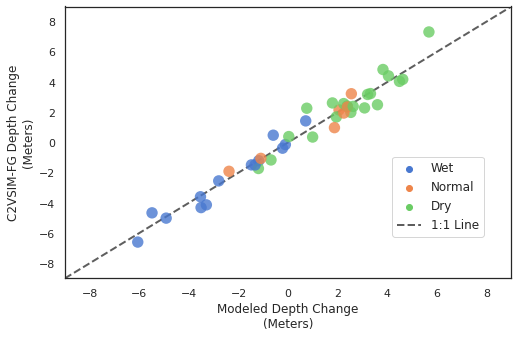
\includegraphics[width=0.5\textwidth]{results_gw_depth_response_calib.png}
    \caption{Results groundwater depth response function and C2VSIM-FG (\cite{dwr_c2vsimfg_2021}). Dots represent the median of each posterior predictive distribution of groundwater depth change, colors represent the water-year type in year t.}
    \label{fig:mesh1}
\end{figure}







\newpage
\printbibliography

\end{document}

\textbf{abstract AGU}


Model    
% $$\Delta GWD \sim Normal(\mu_{i},\sigma)$$

% $$\mu_i = \alpha_{water \, year_{t}[i]} + \gamma_{water\, year_{t-1}[i]} + \beta_{water\, year_{t}[i]}*AGWP_{[i]} + \beta2_{water\, year_{t-1}[i]}*AGWP_{[i]}$$

% $$\alpha_{[i]} \sim Normal(\overline{\alpha},\sigma_{\alpha})$$

% $$\gamma_{[i]} \sim Normal(0,\sigma_{\gamma})$$

% $$\beta_{[i]} \sim Normal(\mu_{\beta},\sigma_{\beta})$$

% $$\beta_{[i]} \sim Normal(0,\sigma_{\beta})$$


% $$\alpha[i] \sim Normal(0,1)$$

% $$\alpha[i] \sim Normal(0,1)$$

% $$\alpha[i] \sim Normal(0,1)$$

% $$\alpha[i] \sim Normal(0,1)$$

\begin{center}
\begin{tabular}{ |c|c|c| } 
 \hline
 Parameter & Description & Source \\ 
 $b_{SW,t}$ & Surface water available for each year t & \cite{zeff_californias_2020} \\ 
 $p_{i,t}$ & Prices by crop i and year t & cell3 \\ 
 cell4 & cell5 & cell6 \\ 
 cell7 & cell8 & cell9 \\ 
 \hline
\end{tabular}
\captionof{table}{Parameters sampled for the stochastic time series and used in the Hydro-economic model}
\end{center}